\chapter{Prototype Solution}
\label{chapter:prototype}

In Section \ref{sec:benchmarking} existing solutions for the problems of
publishing, sharing and managin research data were presented. It is clear that
since these solutions exist, there is no point in reinventing the wheel and
implement a new system. Instead we decided to implement a local installation
of some of the systems presented in the benchmarking section. From the test
installations we would choose the one that worked the best and use that to
run tests on potential users of the system. This way we would get insights
going forward on what the finalized system would look like. It's also notable
that the existing solutions are remarkably similar, so using any one of them
would give appliccable results.

The prototype solution focuses on publishing and sharing of research data. The
other option would have been to focus on the research data management during
the research project, but research projects last longer than the span of this
thesis and the results gained from that would likely be quite superficial.
The lack of culture and practices are a factor for both publishing and
and managing research data. The lacking of research data management culture is
due to the lack of education and need for it, whereas publishing research data
is a moderately new phenomenon. This makes it also a more interesting subject
of study.

We ended up choosing the Harvard Dataverse solution to be the prototype for our
purposes. The follwing sections detail the rationale behind this choice, the
technical details of the system and the tests that were conducted using the
system along with the learnings.

\section{Rationale behind selecting Dataverse}

As a part of the benchmarking the existing solutions and in order to select the
we right tool to run tests on users tried installations of a Hydra head, a
Zenodo instance and a Harvard Dataverse instance. These three were chosen
because they represent different technologies and are widely adopted as tools
for publishing research data.

\subsection{Hydra head installation}

Setting up a Hydra head is fairly simple using Ruby
Gems\footnote{\url{https://github.com/projecthydra/hydra-head}}.
Setting up the basic Hydra head
does not get you far, however, since after setting up the installation you need
to define your data model and almost everything else on your repository.

This setup cost makes Hydra a very versatile framework. It's being used on many
places beyond just research institutions, such as museums and image
repositories\footnote{\url{https://wiki.duraspace.org/display/hydra/Partners+and+Implementations}}.
Many of these systems are built on Hydra solution
bundles\footnote{\url{https://wiki.duraspace.org/display/hydra/Hydra+Solution+Bundles}}
which are also
are open source. Installations of a clean Hydra head and the version
run by Penn State University\footnote{\url{https://scholarsphere.psu.edu/}} were tried.

The conclusion about Hydra heads was that while the system is modern and quite
easy to install, the setup of the system made it too time consuming to setup a
testing prototype in a reasonable time frame. The system is flexible and if you
wanted to build your own customized repository solution Hydra would be suitable
for that. The Penn State implementation was heavily branded and tweaked for
their purposes, making it hard to make it work for ptototyping purposes.
Blacklight\footnote{\url{http://projectblacklight.org/}},
the frontend library used by the Hydra
project, is quite good and makes for easy to use and efficient frontends.

\subsection{Zenodo installation}

We tried installing Zenodo system locally from the source
code\footnote{\url{https://github.com/zenodo/zenodo}}, but could not get the
build process to work correclty as of writing of this thesis.
It was later found out that the Zenodo system, which is built upon the Invenio
archiving software, is notoriously hard to install according to the people who
originally built it\footnote{M. Nurmela and D. Lecarpentier, personal
communication, September 30th, 2015}.

Due to the problems with the installation we ruled the Zenodo system out at
the prototyping phase.

\subsection{Harvard Dataverse}

Harvard Dataverse was easy to install with the installation instructions as
both a development version from the source
code\footnote{\url{http://guides.dataverse.org/en/latest/developers/index.html}} and a
production version with
the installation bundle\footnote{\url{http://guides.dataverse.org/en/latest/installation/}}.

The easy installation immediately gave a functioning software repository to
conduct tests with and that lead to the decision to use Dataverse as the
prototype to test current data repository solutions and gain feedback to plan
ahead.

\subsection{Similarity of the existing solutions}

Though implemented in different technologies, the functioning of the existing
research data repository systems is quite similar. All of them offer form based
dataset uploads, full text searches and some forms of access control. Many of
them are even built on same technologies, such as Solr indexing
software\footnote{\label{solr}\url{http://lucene.apache.org/solr/}} or
postgreSQL\footnote{\label{postgre}\url{http://www.postgresql.org/}}.

The similarity of the systems as well as the fact that there is no global
consensus on what repository software is the best in business hints that you
could use any one of them in your organization. From this angle it also makes
sense to use one of them to gain user insights and figure out how the systems
should be developed in order to gain more users for them.

\section{Users of the system}
\label{sec:users}

As examined in Section \ref{chapter:positioning}, a research data repository
systems have many stakeholders. Identified key stakeholders are presented in
the following:

\begin{itemize}
    \item Research scientists
    \item University courses
    \item Research groups
    \item Librarians
    \item Students
    \item IT staff
    \item Other interested parties
\end{itemize}

The requirements of these different stakeholders were boiled down to user
stories, which are presented in Appendix \ref{chapter:first-appendix}.

\section{System description}
\label{sec:system_description}

Harvard Dataverse is a Java application. Other technologies employed are Apache
Solr\footnotemark[\getrefnumber{solr}] for indexing the database to facilitate search,
postgreSQL\footnotemark[\getrefnumber{postgre}] for database
and Glassfish or Apache for serving the
webpages\footnote{\url{https://glassfish.java.net/}, \url{https://httpd.apache.org/}}.
Dataverse also has in built support for the R statistical computing
language\footnote{\url{https://www.r-project.org/}} for running simple
statistical analyses on the data and for data visualization using the
TwoRavens tool \cite{DBLP:conf/ht/HonakerD14}.

The class model of
Dataverse\footnote{\label{architecture}\url{https://github.com/IQSS/dataverse/tree/4.3/doc/Architecture}}
is described in Figure \ref{fig:dataverse-model}.

\begin{figure}
    \begin{centering}
        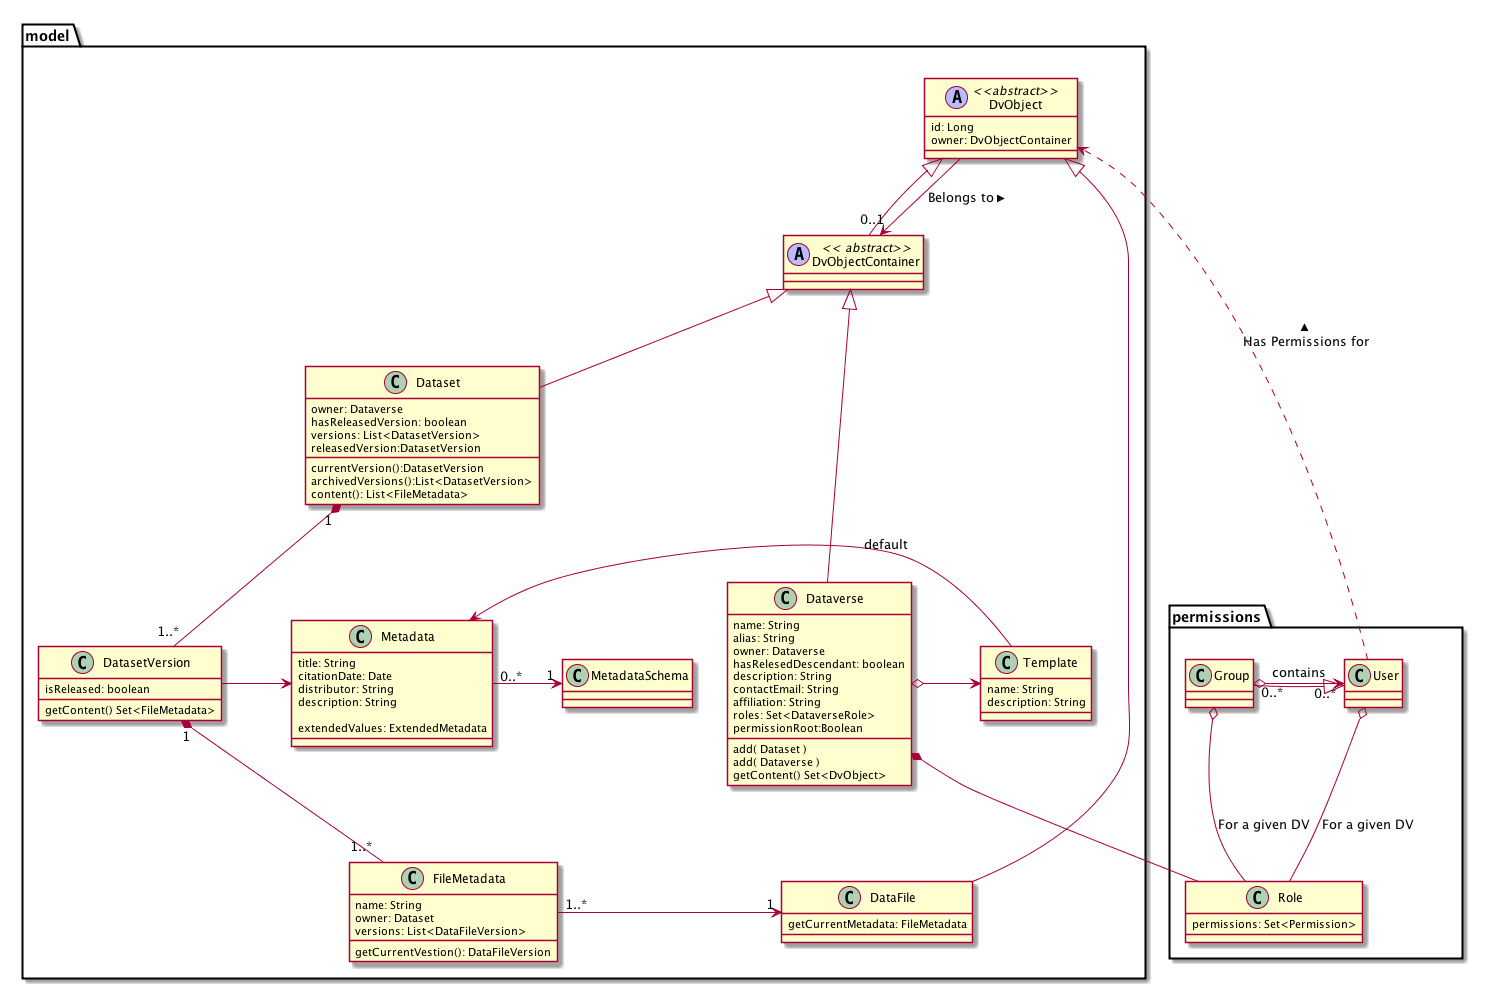
\includegraphics[width=\textwidth]{images/dataverse-model}
    \end{centering}
    \caption[The Dataverse class model]{The Dataverse class model\footnotemark[\getrefnumber{architecture}]}
    \label{fig:dataverse-model}
\end{figure}

In the heart of Dataverse is the division of content into Dataverses. The
closest analogue to a Dataverse is a normal folder in a typical file system -
Dataverses can contain other Dataverses, but in the place of files Datavereses
contain Datasets. Datasets, in turn, contain the files that make up the
dataset. The Dataverse split of the system also allows for fine grained access
control, since Datavereses can be shared with no one, with single users or user
groups.

Users, other than the administrators of the Dataverse, can use the Dataverse
with either the web user interface or the API offered by Dataverse. The
dataflow of using the Dataverse application\footnotemark[\getrefnumber{architecture}] is shown in Figure
\ref{fig:dataflow}.

\begin{figure}
    \begin{centering}
        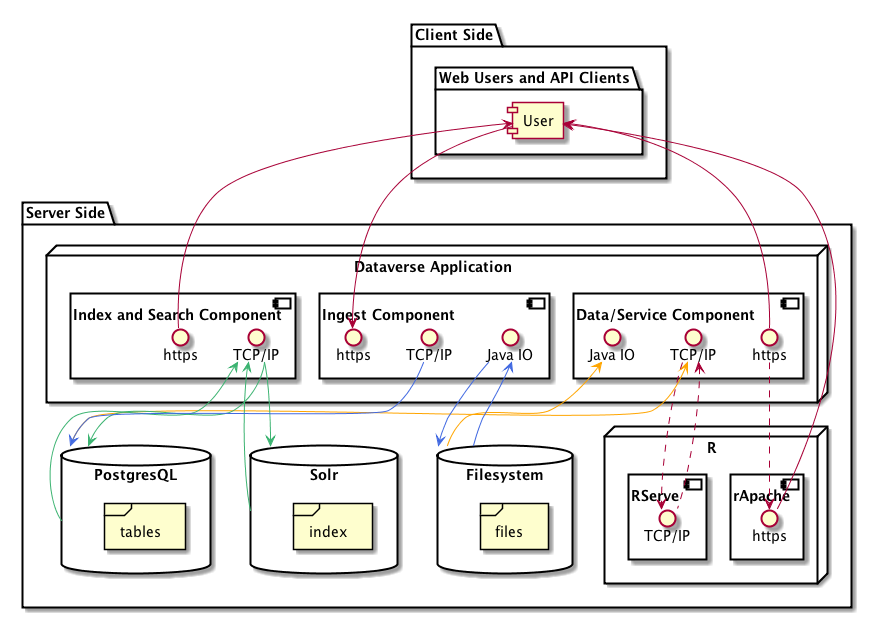
\includegraphics[width=\textwidth]{images/dataflow}
    \end{centering}
    \caption[The Dataverse application dataflow]{The Dataverse application dataflow\footnotemark[\getrefnumber{architecture}]}
    \label{fig:dataflow}
\end{figure}

The Dataverse Java application encompasses the Client Side and Dataverse
Application in Figure \ref{fig:dataflow}. Ingest referers to uploading datasets
to the system and the Index and Search and Data/Service components serve the
user the desired content, be it search results or data to be downloaded. The
rApache component handles the data visualization and runs the TwoRavens tool,
and RServe is used for the statistical computation what the system does.

Two versions of the Dataverse system were installed - one from source
code\footnote{\url{https://github.com/quarian/dataverse}} and one from the
installation bundle provided by the developers of
Dataverse\footnote{\url{https://github.com/IQSS/dataverse/releases/tag/v4.2}}.
The installations were run in the CSC cPouta
environment\footnote{\url{https://research.csc.fi/cpouta}}, which is an
OpenStack instance\footnote{\url{https://www.openstack.org/}}. The source code
installation is referenced from now as the development installation since it
was used to get a feel of the code and the system quality and with the access
to the code if weird situations would come up they could be debugging easier.
The installation from the installation bundle is referred to as the production
installation, since it should be more stable than the branch of development
code that was forked for the development installation. Figure
\ref{fig:cpouta} shows the different installations in the cPouta environment.

\begin{figure}
    \begin{centering}
        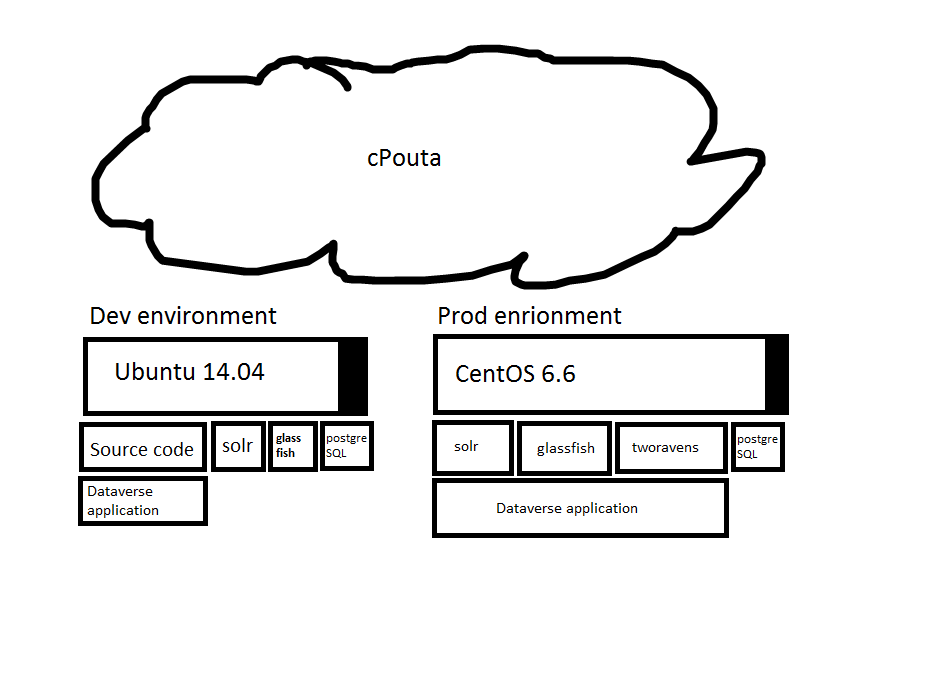
\includegraphics[width=\textwidth]{images/cpouta}
    \end{centering}
    \caption{The different installations in the cPouta environment}
    \label{fig:cpouta}
\end{figure}

The development installation was installed on top of Ubuntu 14.04 and it
worked, even though the installation instrcutions propose the use of Red Hat
based systems. The TwoRavens application was omitted from the development
installation, since the data visualization is not the core functionality of
the reserach data repository software. The production installation was done
on CentOS 6.6, which is a deriavative of Red Hat Linux. The installation was
first tried on CentOS 7.0, but the differences between CentOS 6.x and 7.x made
it so that the installation would not work.

As for the information security of the prototype solution, the development
installation was not set up with any firewall rules or other security, since
its purpose was to get a feel of the system. For the production installation
firewall rules were set using the security groups functions of OpenStack.
When it comes to research data, security is important, and since the
technologies such as Glassfish and postgreSQL are well known software and
their default passwords and ports are well known setting up firewalls and
chanfing those passwords is imperative. Additionally, with Dataverse,
firewalling the port that Apache Solr uses is important, since it circumvents
the user credentials and it could be used to retrieve any indexed information
in the system.

\section{System test setup}
\label{sec:system_testing}

In order to extract value from the prototype Dataverse it needed to be tested
with actual users. Of all the stakeholders presented in Section \ref{sec:users}
the research scientists is the most important one, since without them there is
no research data and without them using the research data repository there is
no public research data. Section \ref{chapter:positioning} summarizes learnings
from the other stakeholder groups. The section also contains results from
surveys conducted on research data management and publishing to provide context
also from the point of view of researcers.

To test this system we worked together with the Complex Newtorks
Group\footnote{\url{http://becs.aalto.fi/en/research/complex\_networks/}} and the
Speech Group\footnote{\url{http://research.ics.aalto.fi/speech/}} of Aalto
University. Two kinds of tests were designed. The first test was a contextual
interview - which means an interview and observation conducted in the user's normal working
environment instead of lab. The contextual interviews were conducted both with
the development installation of the Dataverse as a tool for discussion and as
conversations about the current state of research data management and the
current working practices. The second test was conducted with two lead users
and the production Dataverse installation. The users were asked to input their
datasets to the Dataverse and fill in the appropriate metadata.

The contextual interviews focused on the current methods of research data
management and sharing. The users were asked to describe their practices and
how they had come across to them (taught by the university, learned on their
own or some other methods). When appliccable, the users were asked to show
their current setups for research data management and sharing. When the
development Dataverse was used the users were asked to upload a test dataset
to the Dataverse and walk the interviewer through the thought process. In
addition the interviewees were askes to use the actual Harvard
Dataverse\footnote{\url{https://dataverse.harvard.edu/}} to find datasets
relevant to their field of study and talk through the process. All these
interactions were also observed to find out usability and other issues that
might arise during these exchanges.

The lead users were granted access to the development Dataverse and were
briefly instructed to the different functionalities of Dataverse. The
instructions were left vague in order to make them read the relevant user
guides and provide feedback on how easy the system was to use afer only very
brief instructions. After roughly a month's time the lead users were debriefed
and interviewed about their experiences with the Dataverse system.

The goal of these tests was to understand the current status of research data
management and publishing, how a research data publication system would fit
this status and how well does the research data publication system fill its
designated role.

In addition the installation and maintenance of the prototype installations
would give insight on how the system would be to maintain and how it would work
from a technical point ov view.

\section{Outcomes of the prototype and the tests}
\label{sec:prototype_outcomes}

The contextual interviews and lead user tests yielded results techical matters,
user interface and experience matters and on the current status of the research
data management and publishing.

The results of the tests showed that the technical implementations for research
data sharing fill their role. In the contextual interviews it was clear that
the manual uploading and searching worked fine - the users were able to pick up
the process of searching and uploading datasets. The upload process is form
based, shown in Figure \ref{fig:upload} which is similar to just about any
form based thing you can find onine. Files for datasets can be dragged and
dropped to the user interface or the file browser of the computer and the users
were able to find the suitable method for them. But even
though the upload process is mechanically easy, the upload form contained part
where the user was supposed to insert keywords of the dataset being uploaded.
The keywords come with the concept of vocabulary - which was not known to the
users, as shown in Figure \ref{fig:vocabulary}. In this context vocabulary
refers to a set of words that have been agreed upon within a field of science
in order to standardize communication within the field.

\begin{figure}
    \begin{centering}
        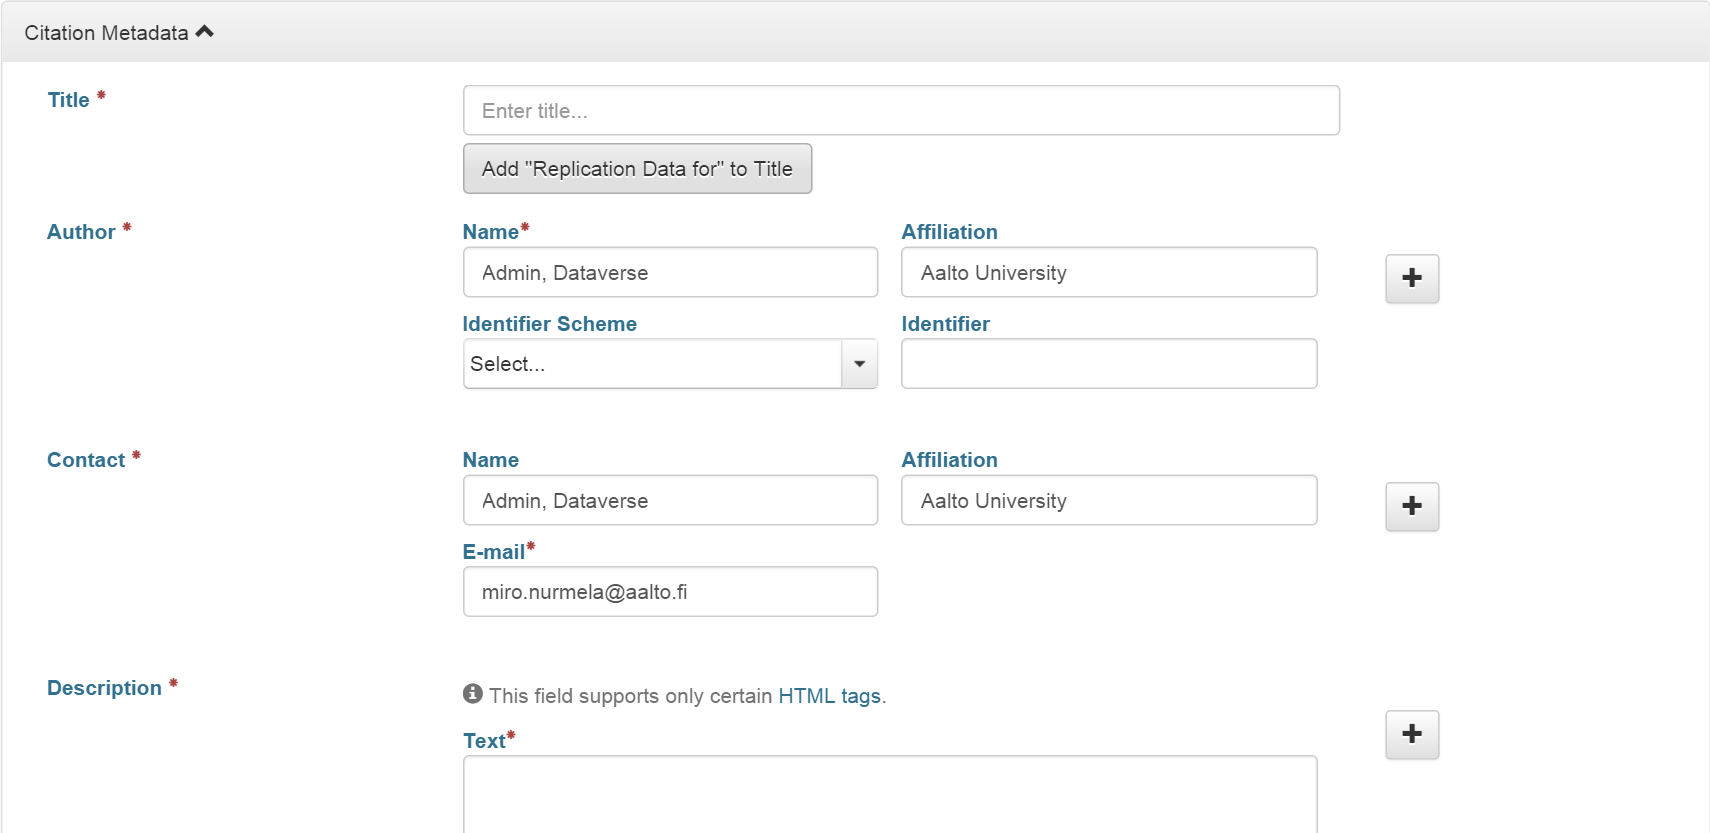
\includegraphics[width=\textwidth]{images/upload}
    \end{centering}
    \caption{A screen capture of the dataset upload form}
    \label{fig:upload}
\end{figure}

\begin{figure}
    \begin{centering}
        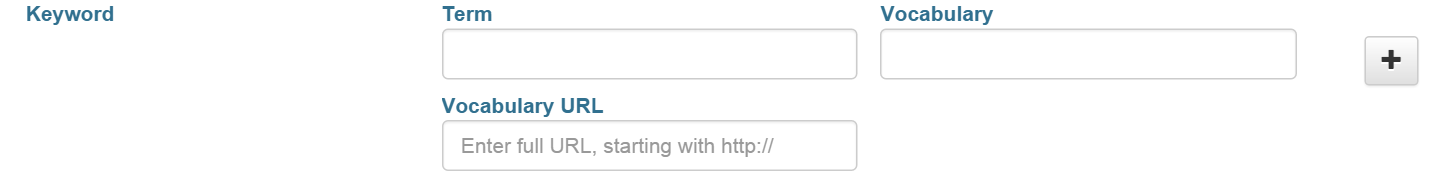
\includegraphics[width=\textwidth]{images/vocabulary}
    \end{centering}
    \caption{A screen capture of the confusion induced vocabulary in the upload form}
    \label{fig:vocabulary}
\end{figure}

What was lacking of the upload process was the extended metadata that would be
important for the reuse of the data. The upload form contains the basic
metadata that is required to make the dataset searchable. Additional metadata,
such as details about the process of gathering the data, needs to be filled in
after the initial upload. The upload form contains a reminder, pictured in
Figure \ref{fig:hint}, to go add the metadata later. This approach has pros and
cons, since it makes the uplaod process easier but makes the metadata likely
lacking. Most users did not notice the hint to go add the metadata later and
those who did notice it did not know where the metadata addition would be done.

\begin{figure}
    \begin{centering}
        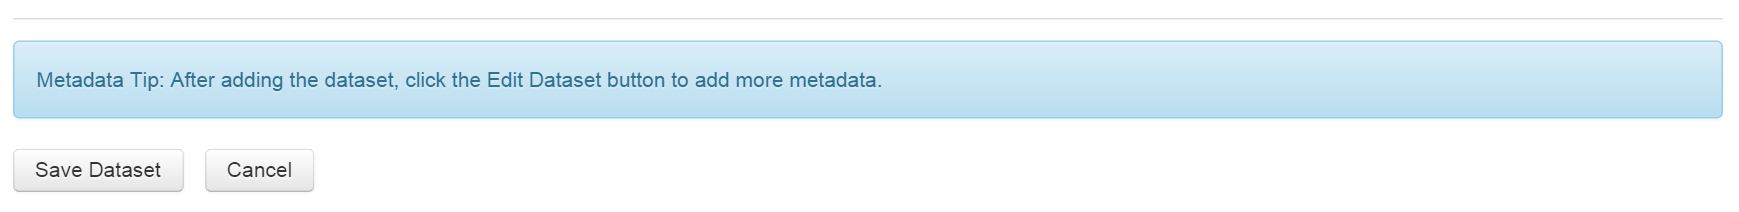
\includegraphics[width=\textwidth]{images/hint}
    \end{centering}
    \caption{A screen capture of the metadata reminder}
    \label{fig:hint}
\end{figure}

The search functionality is placed front and center in the user interface of
the Dataverse main page, as shown in Figure \ref{fig:search_main_page}. Users
easily locate the search bar and are able to start searching for relevant
datasets. The search results leave users lacking, however. This is not entirely
the fault of the search system, since the users found the names and short
descriptions of the datasets poor at describing the datasets which made
finding relevant datasets hard. Using the advanced search, which all the users
did not find, helped to narrow down the options, but the options in the
advanced search were noted to miss details. Details the users were missing
were dataset size and metadata related to their field. It was also clear that
the system worked very well if you knew what you were looking for, for example
a scenario where your fellow researcher would have shared the identifier of
the dataset.

\begin{figure}
    \begin{centering}
        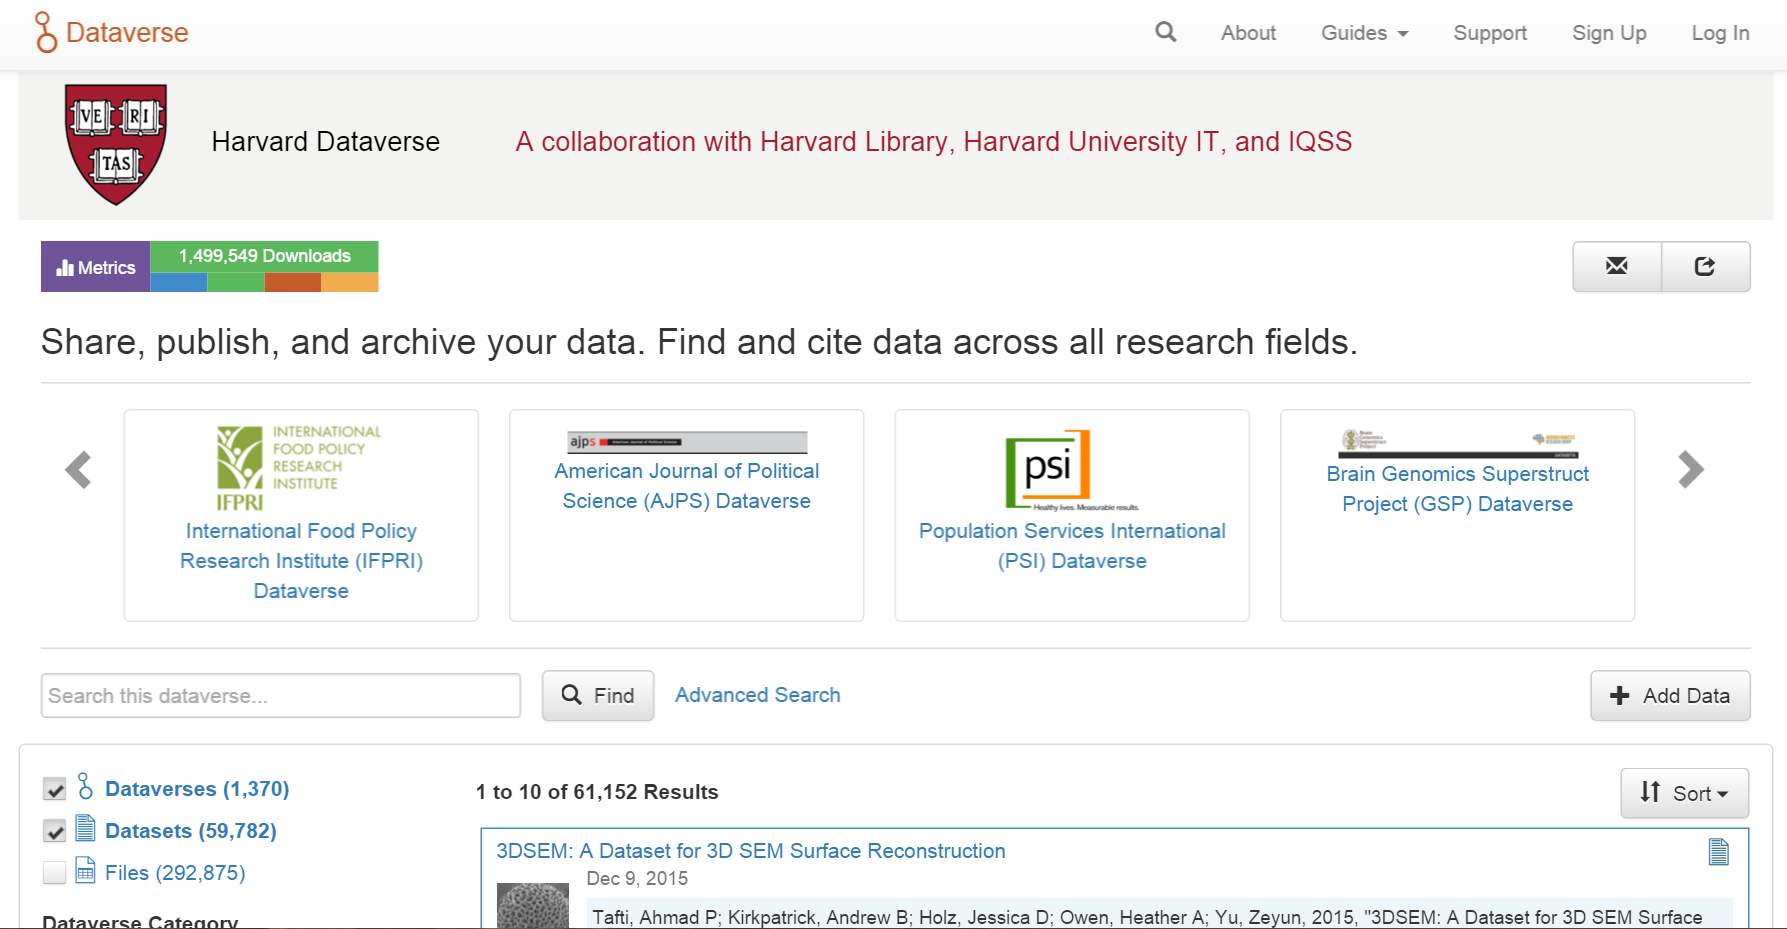
\includegraphics[width=\textwidth]{images/search_main_page}
    \end{centering}
    \caption{A screen capture of the Harvard Dataverse main page}
    \label{fig:search_main_page}
\end{figure}

The order in which the results were displayed was also unclear to the users.
The search results page offers the chance to sort the results, but that option
was missed by all users. The default setting is to sort the results by
relevance, but it is uncelar to what relevance refers to in this context, since
the default search searches all searchable fields in datasets, Dataverses and files.
The fact that Dataverses, datasets and files are by default mixed in the search
results also does not help in finding relevant datasets. There is the option to
filter the files, datasets or Dataverses out of the search results, but the
option was fairly commonly missed by the users. It might be due to the novelty
of the terminology (Dataverse, especially, is a novel concept for the users).

Dataverse implements helpful hovertexts on the terms, as shown in Figure
\ref{fig:hovertext}.

\begin{figure}
    \begin{centering}
        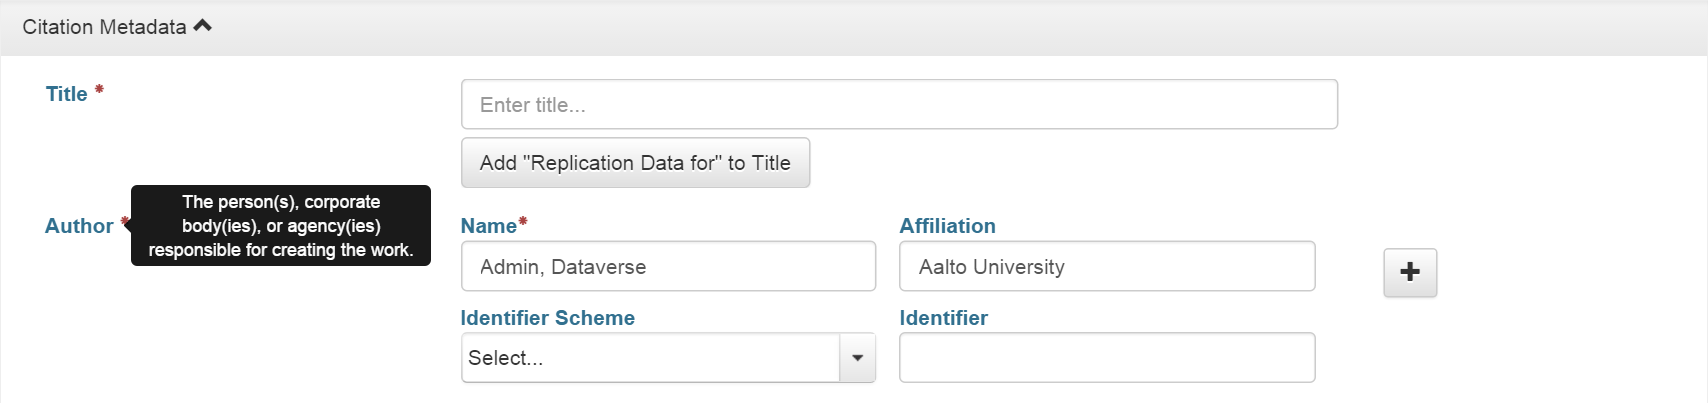
\includegraphics[width=\textwidth]{images/hovertext}
    \end{centering}
    \caption{A screen capture of the hovertexts implemnted in Dataverse}
    \label{fig:hovertext}
\end{figure}



\begin{itemize}
    \item The manual uploading process is just fine
    \item It is a must that there is an API - for example, thousands of video
          files will not be uploaded manually
    \item It is important that the server can cache large files as a part of
          the upload process
    \item Search functionality
        \begin{itemize}
            \item Poorly described datasets
            \item Not intuitive to find data from within all the search results
            \item Dataset size is no available as a search filtering parameter
            \item The vocabulary in advanced search is foreign for the users
            \item The search results are not well organized
        \end{itemize}
    \item Access controls are important and function quite well
    \item Peer to peer teaching would be good
    \item How data is stored (folder structures and such) contains information
          and that should be captured by the system
    \item Accessing data from outside work computers would be nice
    \item More to come here, have to dig up my notes
\end{itemize}
